\chapter{Information Flow Policies for Web Browsers}
\label{ch:webpol}
\blfootnote{The content of this chapter is based on the work published
  as part of the paper,  ``WebPol: Fine-grained Information Flow
  Policies for Web Browsers''~\cite{webpol}}  

Previously proposed approaches~\cite{jsflow,post14,csf15,chudnov-ccs}, 
for enforcing dynamic information flow control in web
browsers lack adequate support for specifying policies
conveniently. Flowfox~\cite{csf14} provides a rich policy framework
but all websites are subject to the same policy, and the underlying IFC
technique, secure multi-execution~\cite{SME}, does not handle shared
state soundly. COWL~\cite{cowl} uses coarse-grained isolation,
allowing scripts' access to either remote domains or the shared state,
but not both. This requires significant code changes when both are
needed simultaneously (see Chapter~\ref{ch:related} for more
details).

This chapter presents {\sys}, a policy framework that allows
a web-page developer to release data selectively to third-party scripts
(to obtain useful functionality), yet control what the scripts can do
with the data. {\sys} policies label
sensitive content (page elements and user-generated events) at source,
and selectively declassify them by specifying where (to which domains)
the content and its derivatives can flow. Host page developers specify
{\sys} policies in JavaScript, a language already familiar to them. 
{\sys} is integrated with the instrumentation of the dynamic IFC
framework for WebKit presented thus far ({\sys} integrates with any
taint-based IFC solution to overcome the shortcomings listed
above). The expressiveness of {\sys} policies is demonstrated through
examples and by applying {\sys} to two real websites. 

\section{Quantifying Information Leaks}
\label{sec:bgqif}

The information released, or the \emph{mutual information}, is
generally quantified as the difference in the entropy, which is a
measure of the adversary's uncertainty, of the sensitive information 
before and after the information is released, i.e.,  
$$\text{mutual information = initial uncertainty - final
  uncertainty}$$ 
Roughly speaking, this amounts to the gain in knowledge of the
adversary about a sensitive value. The adversary computes a probable
initial set of values for the sensitive value. By observing the
information released, the adversary can refine his/her knowledge set
by removing the improbable values.
Various information-theoretic measures have been proposed~\cite{shannon, guessing, 
  smith2009, clarkson2009, csf12GLeakage} for quantifying information
leaks. Many of these measures determine an average worst-case bound on 
the amount of information that a program can leak. 

Clark et al.~\cite{clark} propose an approach to statically 
quantify the amount of information leaked in an imperative language.
An important result that they prove in their work is that the information 
released by a program in a deterministic system is equal to the Shannon 
entropy of the outputs given the public inputs. Thus, for computing the 
information released by a program about a secret, it is enough to compute
the Shannon entropy of the public outputs given the public inputs. 
Another important result is the Shannon's source coding 
theorem~\cite{shannon} that intuitively states that 
if one can associate variable-sized bit-codes with different outputs 
of a program such that the codes are uniquely-decodable, 
then the average of the code-lengths of these codes has been shown 
to be bounded by the Shannon entropy of the outputs of the program. 
The soundness of our approach builds on top of these two results. 
We associate bit-codes with the outputs of the program being analyzed 
and show that these codes are uniquely-decodable. In other words, 
the information release as computed by our approach averaged over 
all executions is bounded by the actual information released by the program.

\lstset{language=HTML}

\section{{\sys} policy model}
\label{sec:model}
{\sys} works on a browser that has already been augmented with IFC
enforcement based on taint tracking.
% Such an enforcement labels all objects internally.
It provides a framework that allows setting labels at
fine-granularity, thus expressing and enforcing rich policies. This
section explains the design of {\sys}. {\sys} prevents under-the-hood
exfiltration of sensitive data that has been provided to third-party
scripts for legitimate reasons. So, third-party scripts are not
trusted but code from the host domain is trusted.
{\sys}'s policies are agnostic to specific channels of leak.  However, 
current IFC enforcements in browsers track only explicit and implicit 
flows. Consequently, leaks over other channels such as timing and
memory-usage are currently out of scope. % As IFC enforcements improve 
% to cover more channels, {\sys}'s policies will extend to them as well.

\subsection{Policies as event handlers}

The first question in the design of {\sys} is who should specify
policies. Since the goal here is to prevent exfiltration of data by
third-party scripts and it is the developer of the host page who
bootstraps the inclusion of scripts and best understands how data on
the page should be used, it is natural and pragmatic to have the
developer specify policies, possibly as part of the page itself.

The next question is how the developer specifies policies. To answer
this, recall the two requirements identified in
Section~\ref{sec:overview} --- it should be possible to specify
different policies on different page elements and policies should be
allowed to include code that is executed on-the-fly to generate
labels. Considering the fact that sensitive data is usually
generated by input events, it is clear that policies should \emph{be}
page element-specific (trusted) code that is executed after events
have occurred (this code labels event-generated data). Fortunately,
web browsers provide exactly this abstraction in the form of event
handlers! So, the event-handling logic in web browsers is extended to
express {\sys} policies. This allows leveraging a lot of the existing
browser logic for event handler installation, parsing and event
dispatch in interpreting policies. The rest of this section explains
how this is done. 
% starting with a brief overview of event handling in web browsers.

% \medskip \noindent \textbf{Event handlers and event dispatch.}
% Browsers execute JavaScript functions, called event handlers, in
% response to input events like mouse clicks, key presses, and
% asynchronous network receives. Save for network receive events, every
% event has a \emph{target}, which is an element in the page's DOM where
% the event originated. For instance, if a button is clicked, the target
% of the ensuing event is the button. Code running on a page can add an
% event handler on any element on the page, listening for a specific
% event. When an event occurs, all handlers associated for that event
% with the event's target and the target's ancestors are triggered
% sequentially. This is called \emph{event dispatch.} The specific order
% in which handlers are triggered is not relevant for our purposes
% (although it is fairly interesting for IFC
% enforcement~\cite{csf15}). The whole process is bootstrapped by the
% static HTML of the page, which may contain JavaScript that is executed
% when the page loads initially, and this JavaScript installs the first
% set of event handlers.

% \medskip \noindent \textbf{Policy handlers.}
In {\sys}, policies are special event handlers, specified using a
special marker in the HTML source of the hosting page. These special
handlers, called \emph{policy handlers}, follow standard JavaScript
syntax, can be attached to any page element, listening for any event
and, like other handlers, are triggered every time the event is
dispatched on the element or any of its descendants. However, unlike
other handlers, the sole goal of policy handlers is to assign labels
to other sensitive objects, including the event being dispatched. To
allow the policy handlers to do this, the browser is slightly modified 
to afford these handlers two special privileges:
\begin{itemize}
\item Policy handlers can execute two new JavaScript API functions
  that set labels on other objects. No other JavaScript code can
  execute these two functions. These functions are described later.
\item During event dispatch all applicable policy handlers are executed
  before ordinary handlers. This ensures that labels are set before
  ordinary handlers (including those of third-party scripts) execute.
\end{itemize}
To maintain the integrity of the policies, policy handlers must be
included in the HTML source of the page directly. They \emph{cannot}
be installed dynamically by JavaScript code. Otherwise, third-party
scripts could install policy handlers that set very permissive labels.
Also, if a DOM element has a policy handler, third-party scripts are
disallowed from detaching that element or moving it elsewhere, as that 
can change the interpretation of the policy. Similarly, changing the
attributes of such an element is restricted.

\begin{figure}[tb]
  \centering 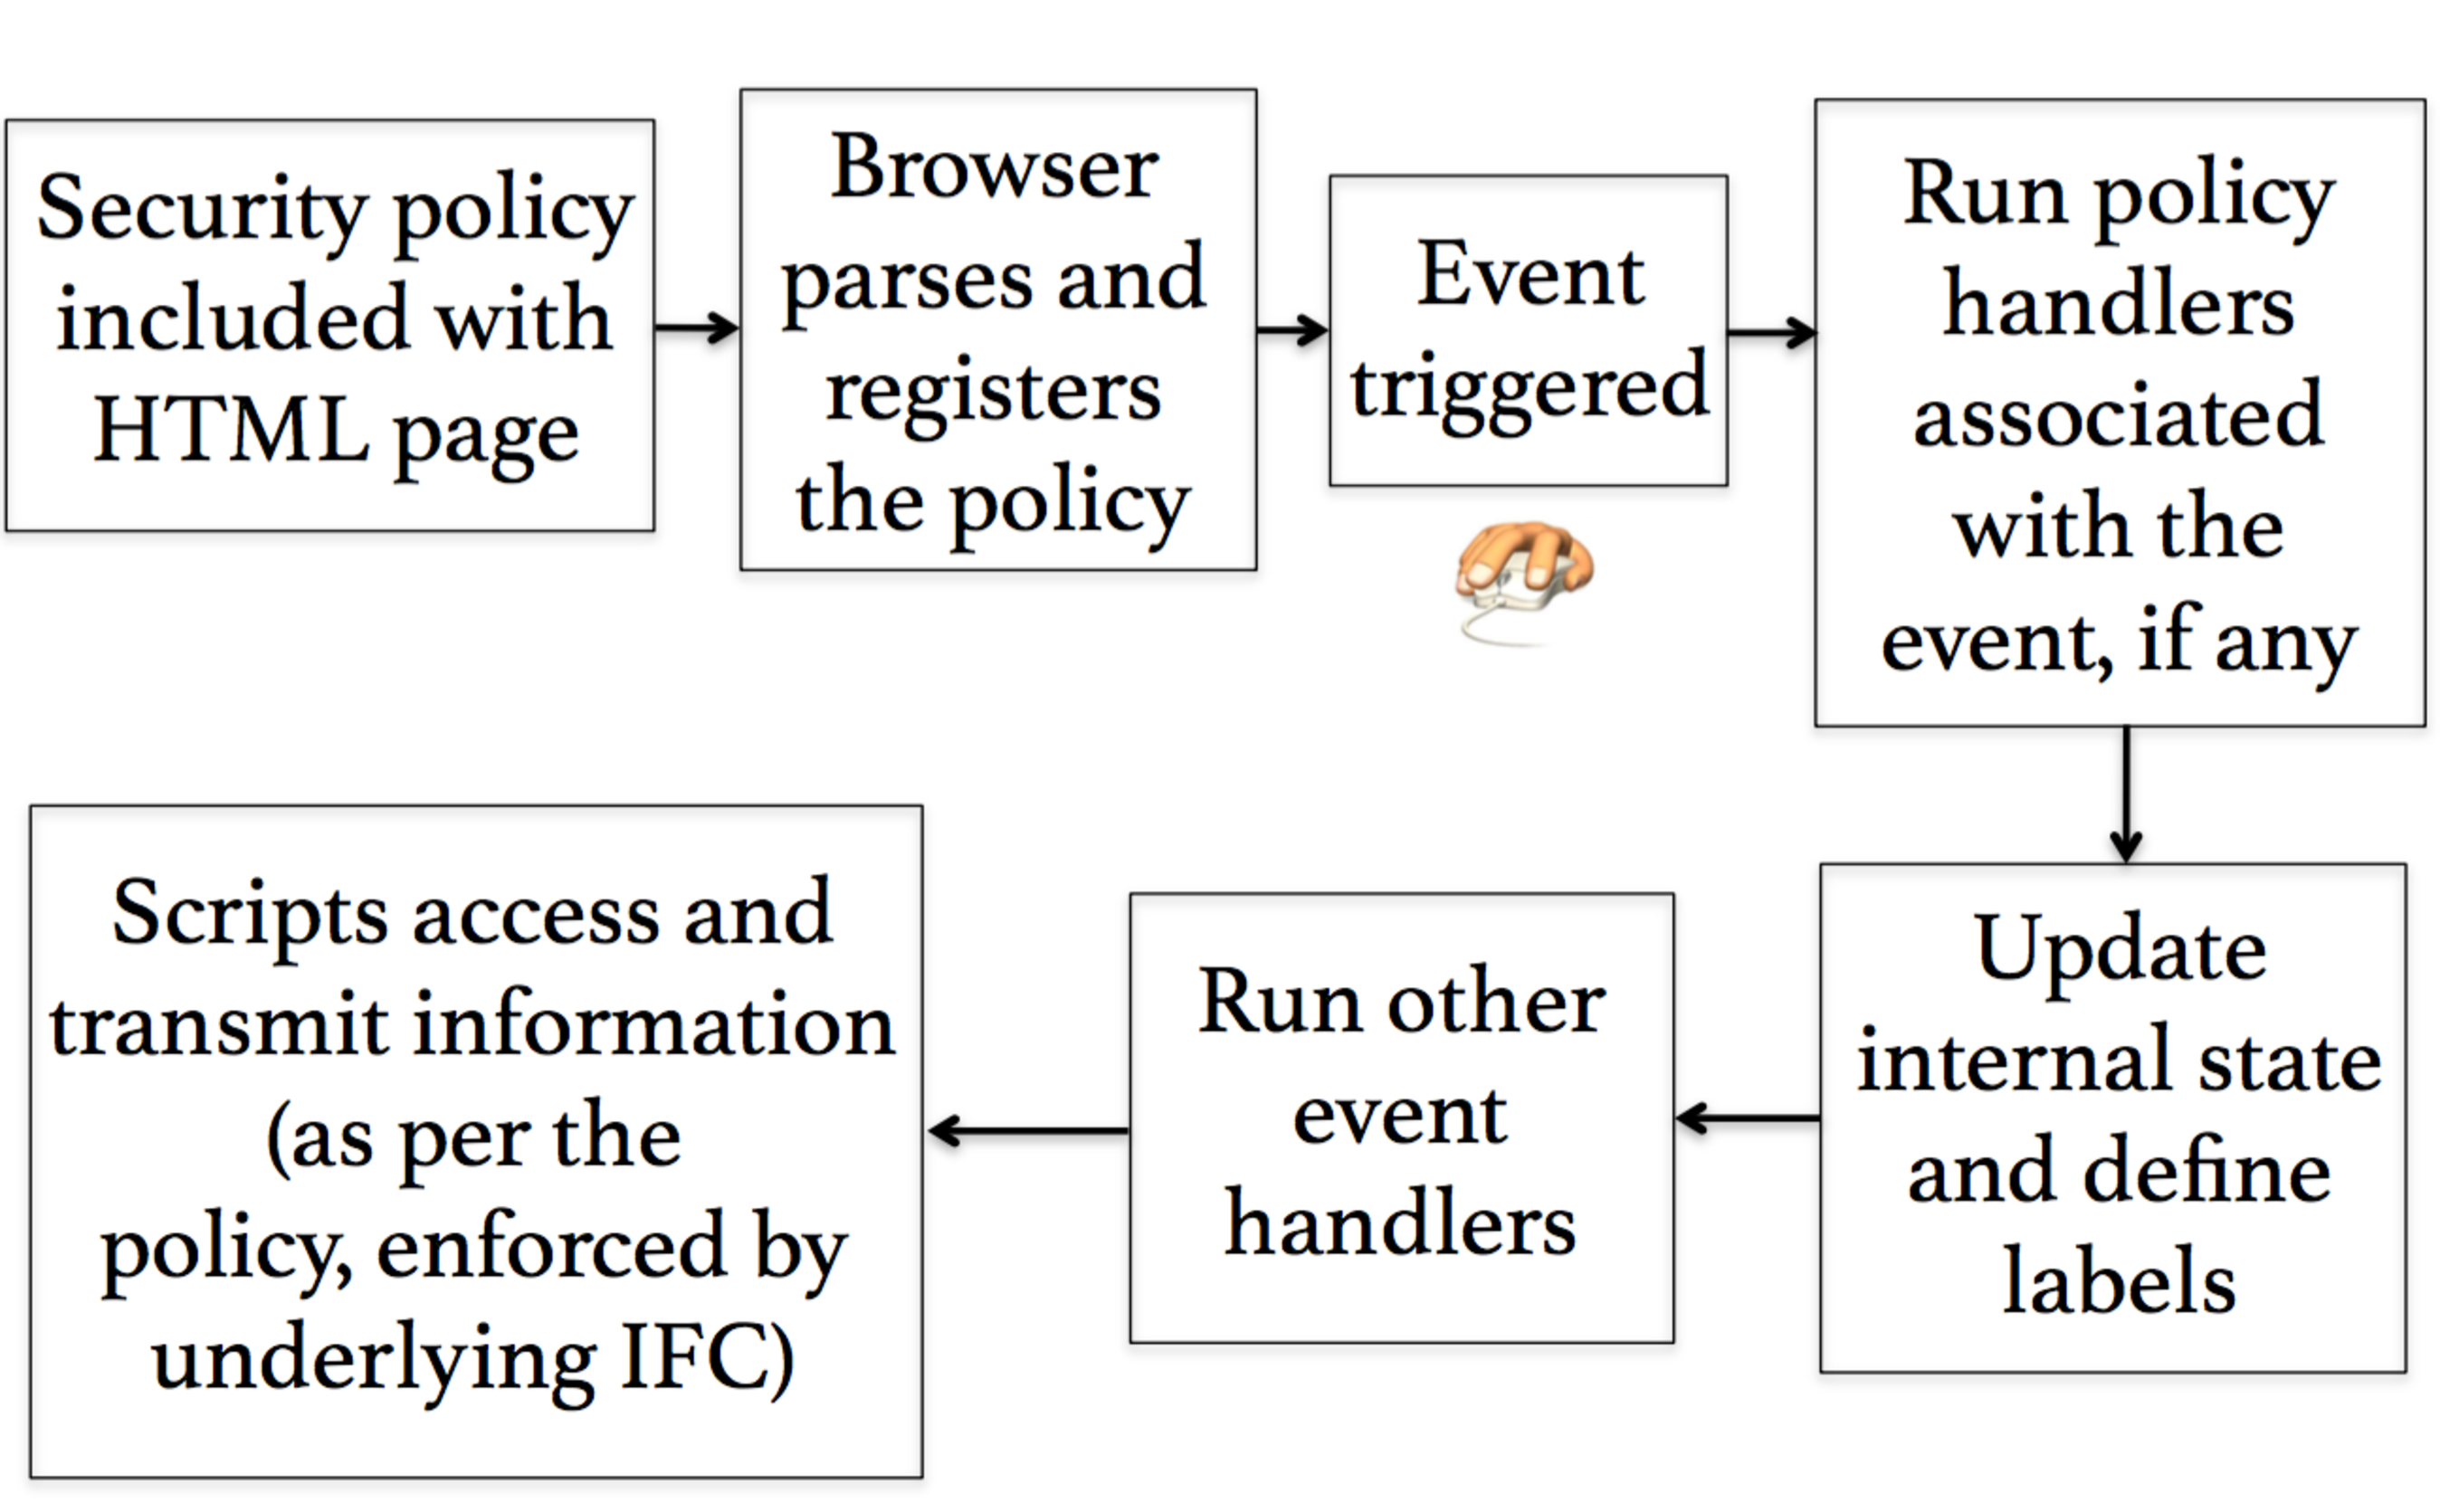
\includegraphics[width=8cm]{chapters/browser/webpol/Model.pdf} \caption{Workflow
  of the {\sys} policy model} \label{fig:model}
\end{figure}

Since different policy handlers can be associated with different
elements, Requirement~1 is satisfied.  Moreover, policy handlers are
ordinary JavaScript code, so they can also maintain local state in
private variables, thus satisfying Requirement~2. 

The workflow of policy interpretation in {\sys} is shown in
Figure~\ref{fig:model}. Briefly, the steps are:

\begin{enumerate}
\item The web page developer specifies the policy in the host HTML
  page in the form of special event handlers.
\item The browser parses the policy and registers its handlers (mostly
  like usual handlers, but with the two special privileges mentioned
  above).
\item When an event dispatches, listening policy handlers are
  executed first.
\item These policy handlers set labels on objects affected by the
  event, including the event object itself. They may also
  update any local state they maintain.
\item The remaining event handlers are dispatched as usual.
  The IFC enforcement in the browser enforces all labels that have
  been set by the policy handlers (during any prior event's dispatch),
  thus preventing any data leak in contravention of the labels.
\end{enumerate}

\subsection{Integration with the web browser}

{\sys} needs minor modifications to the browser to parse and interpret
policies and to expose additional JavaScript API functions to set
labels.

\medskip \noindent \textbf{HTML and event dispatch changes.}
{\sys} adds an HTML extension to differentiate policy code from other
JavaScript code. Concretely, the browser's parser is changed to
interpret any script file with the extension \texttt{.policy} included
directly in the host page as a policy. If such a \emph{policy script}
installs a handler, it is treated as a policy handler. Additionally, a
policy script can set labels on the page's global variables and DOM
elements (like password fields). If a script does this, it should be
included in the host page before third-party scripts that use those
variables. {\sys} also requires a small change to the browser's event
dispatch mechanism to execute policy handlers before other handlers.

\medskip \noindent \textbf{Label-setting APIs.}
{\sys} exposes two new JavaScript API functions to set labels. These
functions can be called only by the policy code in \texttt{.policy}
files and handlers installed by such files (the browser is modified to
enforce this).

The function \texttt{setLabel(label)} sets the label of the object on
which it is called to \texttt{label}. As explained
earlier, \texttt{label} can be \texttt{public}, a domain name,
or \texttt{local} (the default is \texttt{public}). Once an object's
label is set, it is enforced by the underlying IFC enforcement. The
special label \texttt{HOST} is a proxy for the domain of the host
page.

The function \texttt{setContext(label)} can be called only on an event
object. It restricts the \emph{visibility} of the event to
label \texttt{label} and higher. In simple terms, if \texttt{label} is
a domain, then only that domain can ever learn that this event
occurred, whereas if \texttt{label} is \texttt{local}, then no domain
can ever learn that this event occurred. Technically, this is
accomplished by setting the $\pc$ of the 
event handlers running during the dispatch to \texttt{label}, which
ensures that their side-effects (writes to DOM and network
communication) are labeled \texttt{label} or higher.

As opposed to \texttt{setLabel}, which makes individual data objects
(like password fields) private, \texttt{setContext} makes the
\emph{existence} of an event private. This is useful.
For instance, clicking on the ``politics'' section of a news feed
might indicate that the user is interested in politics, which may be
private information, so the page may want to hide even the existence
of click events from third-party scripts. (The distinction between the
privacy of event content and event occurrence has been previously
described by Rafnsson and Sabelfeld~\cite{Rafnsson-csf13}.)


\section{Expressiveness of {\sys}}
\label{sec:examples}

The expressiveness of {\sys} policies is illustrated through the
following examples.

\begin{lstlisting}[float, caption=Password strength checking script that leaks the password,label=egscript1,language=C]
var p = document.getElementById("pwd");
p.addEventListener("keypress", function (e){
  var score = checkPwdStrength(p.value);
  document.getElementById("pwdStrength").innerText = score; 
  new Image().src = "http://stealer.com/pwd.jsp?pwd="+p +score;
});
\end{lstlisting}

\subsection{Example 1: Password strength checker}  
Many websites deploy \emph{password strength checkers} on pages where
users set new passwords. A password strength checker is an event
handler from a third-party library that is triggered each time the
user enters a character in the new password field. The handler
provides visual feedback to the user about the strength of the
password entered so far. Strength checkers usually check the length of
the password and the diversity of characters used. Consequently, they
do not require any network communication. However, standard browser
policies cannot enforce this and the password strength checker can
easily leak the password if it wants to. Listing~\ref{egscript1} shows
such a ``leaky'' password checker. The checker installs a listener for 
keypresses in the password field (line 2). In response to every
keypress, the listener delivers its expected functionality by checking
the strength of the password and indicating this to the user (lines 3,
4), but then it leaks out the password to \texttt{stealer.com} by
requesting an image at a URL that includes the password (lines 5, 6). 

With {\sys}, the developer of the host web-page can prevent any
exfiltration of the password by including the policy script:

\medskip
\texttt{document.getElementById("pwd").setLabel("HOST");}

\medskip 
\noindent This policy sets the label of the password field to the
host's own domain using the function
\texttt{setLabel()}. Subsequently, the IFC enforcement restricts all
outgoing communication that depends on the password field to the host.

Conceptually, this example is simple because it does not really
leverage the fine-granularity of {\sys} policies and fine-grained
dynamic IFC. Here, the third-party script does not need any network
communication for its intended functionality and, hence, simpler
confinement mechanisms that prohibit a third-party script from
communicating with remote servers would also suffice. The next example 
is a scenario where the third-party script legitimately needs remote
communication, which leverages the fine-granularity of {\sys} policies
and fine-grained dynamic IFC.

\begin{lstlisting}[float, caption=Currency converter script that leaks a private amount,label=egcc,escapechar=\%]
function currencyConverter() {
	var toCur = document.getElementById("to").value;
	var xh = new XMLHttpRequest();
	xh.onreadystatechange = function() { %\label{startcallback}%
		if (xh.readyState == 4) { %\iffalse && xhttp.status == 200 \fi %
			currencyRate = eval(xhttp.responseText);%\label{startsend}%
			var aAmt = document.getElementById("amt").value;
			var convAmt = aAmt * currencyRate;
			document.getElementById("camt").innerHTML = convAmt;%\label{ressend}%
			xh.open("GET","http://currConv.com/amount.jsp?atc=" + aAmt);%\label{endsend}%
			xh.send(); }} %\label{endcallback}%
	xh.open("GET","http://currConv.com/conv.jsp?toCur=" + toCur, true);
	xh.send(); }
\end{lstlisting}


\subsection{Example 2: Currency conversion}
Consider a web-page from an e-commerce website which displays the cost
of an item that the user intends to buy. The amount is listed in the
site's native currency, say US dollars (USD), but for the user's
convenience, the site also allows the user to see the amount converted
to a currency of his/her choice. For this, the user selects a currency
from a drop-down list. A third-party JavaScript library reads both the
USD amount and the second currency, converts the amount to the second
currency and inserts it into the web-page, next to the USD amount.
%
The third-party script fetches the current conversion rate from its
back-end service at \texttt{currConv.com}. Consequently, it must send
the \emph{name} of the second currency to its back-end service, but
must not send the amount being converted (that is private
information). The web browser's same-origin policy has been relaxed
(using, say, CORS~\cite{cors}) to allow the script to talk to its
back-end service at \texttt{currConv.com}. The risk is that the script
can now exfiltrate the private amount. Listing~\ref{egcc} shows a
leaky script that does this. On line~\ref{endcallback}, the script
makes a request to its back-end service passing to it the two
currencies. The callback handler (lines
\ref{startcallback}--\ref{endcallback}) reads the amount from the page
element \texttt{amt}, converts it and inserts the result into the page
(lines \ref{startsend}--\ref{ressend}). Later, it leaks out the amount
to the back-end service on line~\ref{endsend}, in contravention of the
intended policy.

With {\sys}, this leak can be prevented with the following policy that
sets the label of the amount to the host only:

\medskip
\texttt{document.getElementById("amt").setLabel("HOST")}

\medskip
\noindent This policy will prevent exfiltration of the amount and will not
interfere with the requirement to exfiltrate the second
currency. Importantly, no modifications are required to a script that
does not try to leak data (e.g., the script obtained by dropping the
leaky line~\ref{endsend} of Listing~\ref{egcc}).

\begin{lstlisting}[float,caption=Policy that allows counting clicks but hides details of the clicks,label=eganal1]
var p = document.getElementbyId("sect_name");
p.addEventListener("click",function(event){
  event.setLabel("HOST"); });
\end{lstlisting}

\subsection{Example 3: Web analytics} 
To better understand how
users interact with their websites, web developers often include
third-party analytics scripts that track user clicks and keypresses to
generate useful artifacts like page heat-maps (which part of the page
did the user interact with most?). Although a web developer might be
interested in tracking only certain aspects of their users'
interaction, the inclusion of the third-party scripts comes with the
risk that the scripts will also record and exfiltrate other private
user behavior (possibly for monetizing it later). Using {\sys}, the
web developer can write precise policies on which user events an
analytics script can access and when. Several examples of this are
shown. 

\begin{lstlisting}[float, caption=Analytics script that counts clicks,label=egan]
clickCount = 0;
var p = document.getElementbyId("sect_name");  
p.addEventListener("click",function (e){ clickCount += 1; });
\end{lstlisting}

To allow a script to only count the number of occurrences of a class
of events (e.g., mouse clicks) on a section of the page, but to hide
the details of the individual events (e.g., the coordinates of every
individual click), the web developer can add a policy handler on the
top-most element of the section to set the label of the individual
event objects to \texttt{HOST}. This prevents the analytics script's
listening handler from examining the details of individual events, but
since the handler is still invoked at each event, it can count their
total number. Listings~\ref{eganal1} and~\ref{egan} show the policy
handler and the corresponding analytics script that counts clicks in a
page section named \texttt{sect\_name}.

\begin{lstlisting}[float,caption=Policy that only tracks whether a click
  happened or not,label=eganal2]
var alreadyClicked = false;
var p = document.getElementById("sect_name");
p.addEventListener("click",function (event){
  if (alreadyClicked = true) 
     event.setContext("HOST");
  else {
     alreadyClicked = true; 
     event.setLabel("HOST");
}});
\end{lstlisting}

Next, consider a restriction of this policy, which allows the
analytics script to learn only whether or not \emph{at least one}
click happened in the page section, completely hiding clicks beyond
the first. This policy can be represented in {\sys} using a local
state variable in the policy to track whether or not a click has
happened and the function \texttt{setContext()}. Listing~\ref{eganal2}
shows the policy. The policy uses a variable \texttt{alreadyClicked}
to track whether or not the user has clicked in the section. Upon the
user's first click, the policy handler sets the event's label to the
host's domain (line~8). This makes the event object private but allows
the analytics handler to trigger and record the occurrence of the
event. On every subsequent click, the policy handler sets the event's
\emph{context} to the host domain using \texttt{setContext()}
(line~5). This prevents the analytics script from exfiltrating any
information about the event, including the fact that it occurred.

Finally, note that a developer can subject different page sections to
different policies by attaching different policy handlers to them. The
most sensitive sections may have a policy that unconditionally sets
the event context to the host's, effectively hiding all user events in
those sections. Less sensitive sections may have policies like those
of Listings~\ref{eganal2} and~\ref{eganal1}. Non-sensitive sections
may have no policies at all, allowing analytics scripts to see all
events in them.

\begin{lstlisting}[float, caption=Example policy to prevent overlay-based
  stealing of keystrokes,label=overlay,language=C]
document.body.addEventListener("keypress", function (event){
    var o = window.getComputedStyle(event.target).getPropertyValue("opacity");
    if (o < 0.5) 
         event.setLabel("HOST");
});
\end{lstlisting}

\subsection{Example 4: Defending against overlay-based attacks}
To bypass {\sys} policies, an adversarial script may ``trick'' a user
using transparent overlays. For example, suppose a script wants to
exfiltrate the contents of a password field that is correctly
protected by a {\sys} policy. The script can create a transparent
overlay on top of the password field. Any password the user enters
will go into the overlay, which \emph{isn't} protected by any policy
and, hence, the script can leak the password.

Such attacks can be prevented easily in {\sys} using a \emph{single}
policy, attached to the top element of the page, that labels data
entered into all significantly transparent overlays as
\texttt{HOST}. Listing~\ref{overlay} shows such a policy. This
particular policy labels all keypress events on elements of opacity
below $0.5$ as \texttt{HOST}, thus preventing their exfiltration. The
threshold value $0.5$ can be changed, and the policy can be easily
extended to other user events like mouse clicks.

\subsection{Summary of {\sys} expressiveness} 
The security community has extensively studied several
aspects of policy labeling, colloquially called the \emph{dimensions
  of declassification} (see~\cite{dimDecl} for a survey). Broadly
speaking, {\sys} policies cover three of these dimensions---the
policies specify what data is declassified (dimension: what), to which
domains (dimension: to whom) and under what state (dimension:
when). ``What data is declassified'' is specified by selectively
attaching policies to elements of the page. ``Which domains get
access'' is determined directly by the labels that the policy
sets. Finally, labels generated by policy handlers can depend on
state, as illustrated in Listing~\ref{eganal2}.

There are two other common dimensions of labeling---who can label the
data (dimension: who) and where in the code can the labels change
(dimension: where). These dimensions are fixed in {\sys} due to the
specifics of the problem: All policies are specified by the host page
in statically defined policies.


